\section{Metody krokowe dla n-D (stepping methods in many variables)}

\subsection{Przeszukiwanie losowe}

  \begin{frame}{Przeszukiwanie losowe} %frame - granice slajdu

    \begin{block}{}
 	  \begin{itemize} % itemize - granice punktowania
 		\item[--] szukanie na siatce dla $n > 2$ - bez sensu \emph{(grid search)} % emph - kursywa
 		\item[--] doświadczenie z całkowania $\rightarrow$ mogą być tu też przydatne metody Monte-Carlo % item - pojedyncze wypunktowanie
 	  	\item[--] $\vec{x_i}$ - wybierane losowo, zgodnie z rozkładem: % $ .. $ - tekst matematyczny
 	  	\begin{itemize}
 		  \item równomiernym,
 		  \item normalnym
 	  	\end{itemize}
 	  	\item[--] o środku w najlepszym ze znalezionych punktów,
 	  	\\przy zadanej szerokości.
 	  	\item[--] stosowane, gdy: % \\ - złamanie linii
 	  	\begin{itemize}
 		  \item nic nie wiadomo o $F(x)$,
 		  \item $F(x)$ ma kilka minimów,
 		  \item dla ustalenia rozsądnego punktu startowego
 	  	\end{itemize}
 	  \end{itemize}
 	\end{block}

  \end{frame}

\subsection{Zmiana jednego parametru (single parameter variation)}

  \begin{frame}{Zmiana jednego parametru cz.1}

	Warunek na istnienie minimum - \emph{stacjonarny punkt} $ x_i $,
	\\tj. \emph{znikanie wszystkich $ n $ pochodnych} $ \frac{\partial F}{\partial x_i} $ , $ i = 1,2,3,\ldots ,n $
	\begin{figure}
		\centering
		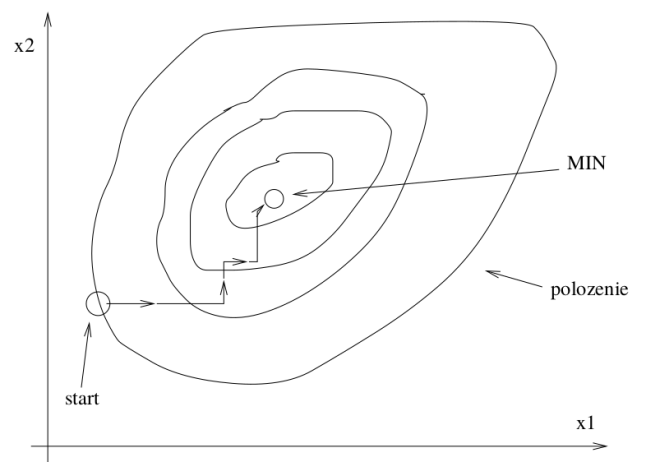
\includegraphics[height=0.6\textheight ,width=0.8\textwidth]{img/17/change_param_1}
	\end{figure}

  \end{frame}

  \begin{frame}{Zmiana jednego parametru cz.2}

	Niebezpieczna - przypadki z wąwozem (narrow valley)
	\begin{figure}
		\centering
		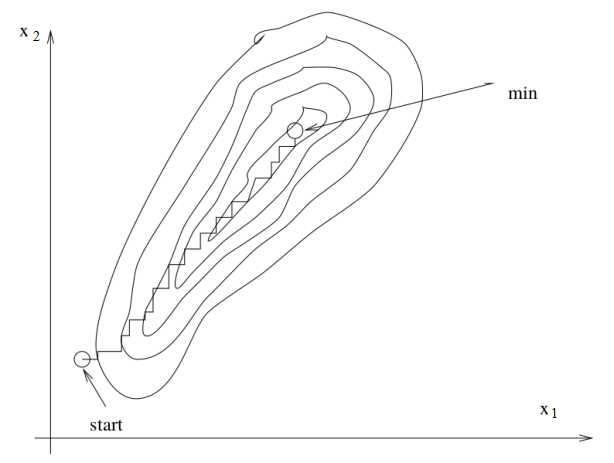
\includegraphics[height=0.6\textheight ,width=0.8\textwidth]{img/17/change_param_2}
	\end{figure}
	w tym przypadku - stosowane ulepszone metody

  \end{frame}

\subsection{Metoda Rosenbrocka}

  \begin{frame}{Metoda Rosenbrocka}

    \begin{block}{Algorytm}
 	  \begin{itemize}
 		\item wykonuje się jeden pełny cykl minimalizacji wzgl. kolejno wszystkich parametrów (współrzędnych),
 		\item zmiana osi układu współrzędnych - nowy układ ortogonalny:
 		\\jedna z osi od punktu początkowego do końcowego
 		\\w ostatnim cyklu minimalizacji,
 		\item nowy cykl \ldots $\rightarrow$ w nowym układzie współrzędnych
  	  \end{itemize}
  	\end{block}
  	  Niestety $\rightarrow$ metoda mało efektywna dla dużego $n$
  	  \\(w połączeniu z metodą aproks. kwadratowej)

  \end{frame}

\subsection{Metoda simpleksów}

  \begin{frame}{Simplex - wprowadzenie}

    \begin{block}{Definicja}
 	  \textbf{Simplex} - najprostsza $n$-wymiarowa figura określona przez $(n+1)$ wierzchołków (vertex).
  	\end{block}
  	\begin{figure}
		\centering
		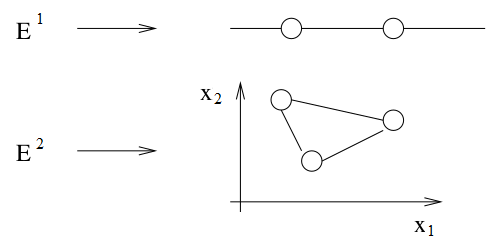
\includegraphics[height=0.3\textheight ,width=0.5\textwidth]{img/17/simplex}
	\end{figure}
  	\begin{block}{}
 	  \textbf{Nazwa metody} - w każdym kroku informacja o funkcji dotyczącej jej wartości w $n+1$ punktach
  	\end{block}

  \end{frame}

  \begin{frame}{Opis metody cz.1}

  	\begin{figure}
		\centering
		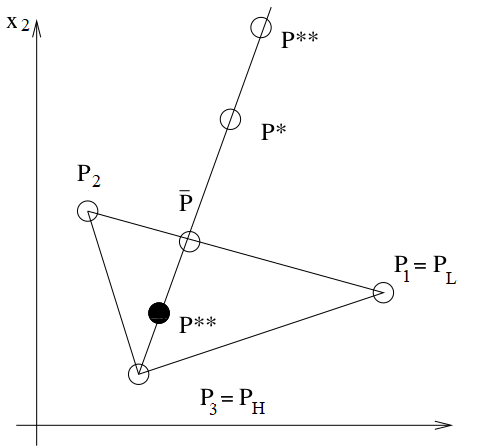
\includegraphics[height=0.8\textheight ,width=0.8\textwidth]{img/17/simplex_method}
	\end{figure}

  \end{frame}

  \begin{frame}{Opis metody cz.2}

	\begin{enumerate}
		\item Wybieramy (losowo, min 1-D) 3 punkty $P_1,P_2,P_3$
		\\i wyznaczamy w nich
		\\ $F(x): P_H \rightarrow F(x)$ - największa (highest)
		\\ $P_L \rightarrow F(x)$ - najmniejsza (lowest)
		\item Wyznaczamy "środek masy" wszystkich punktów
		\\z pominięciem $P_H$
		  \begin{displaymath}
		    \overline{P}=\frac{1}{n}\left[\sum_{i=1}^{n+1}P_i-P_H\right]
		  \end{displaymath}
		\item Obliczamy odbicie $P_H$ wzgl. $\overline{P} : P$* $= \overline{P}+(\overline{P}-P_H)$ jeżeli
		\\ $F(P$*$) < F(P_L) \Rightarrow$ nowy $P$** $= \overline{P}+2*(\overline{P}-P_H)$
		\\ $F(P$*$) > F(P_L) \Rightarrow$ nowy $P$** $= \overline{P}-1/2*(\overline{P}-P_H)$
		\newcounter{saveenumi}	% do kontynuacji numeracji na następnym slajdzie
		\setcounter{saveenumi}{\value{enumi}}
	\end{enumerate}

  \end{frame}

  \begin{frame}{Opis metody cz.3}

	\begin{enumerate}
		\setcounter{enumi}{\value{saveenumi}}
		\item Punkt $P_H$ zastępujemy przez najlepszy z $P$* i $P$**
		\smallskip
		\\Jeżeli żaden z nowych punktów nie jest lepszy od $P_H$, tworzymy simplex oparty o $P_L$ w wymiarach $0.5$ $*$ poprzednie
	\end{enumerate}
	Inne możliwości:
	\begin{itemize}
		\item współczynniki $\neq 2$ oraz $\neq \frac{1}{2}$,
		\item interpolacja kwadratowa wzdłuż prostej $(P_H,\overline{P})$
	\end{itemize}
	\begin{block}{}
	  	\textbf{Uwaga!}
 	  	\\nowy punkt nie może być zbyt blisko $\overline{P}$ - bo to grozi redukcją
 	  	\\(bez powrotu) simpleksów w $n$ do hiperpłaszczyzny
    \end{block}

  \end{frame}

  \begin{frame}{Opis metody cz.4}

	\begin{block}{Zalety :}
	  	\begin{itemize}
	  		\item[--] nieczuła na płytkie minima
	  		\\(pochodzenia: zaokrąglenia, statystyka \ldots),
	  		\item[--] mała ilość obliczeń funkcji $F(X)$ w każdym kroku,
	  		\item[--] największe możliwe kroki,
	  		\item[--] rozsądny kierunek poszukiwań,
	  		\item[--] bezpieczna i szybka daleko od minimum,
	  		\item[--] daje estymaty błędów parametrów
	  	\end{itemize}
    \end{block}
    \begin{block}{Zbieżność}
	  	$\underbrace{EDM}_{ \text{estimated distance to minimum}} = F(P_H) - F(P_L) < \underbrace{EPSI}_{(\epsilon)}$
    \end{block}

  \end{frame}

\subsection{Metody gradientowe}

  \begin{frame}{Metody gradientowe}

 	$\rightarrow$ w oparciu o informacje o funkcji w małych obszarach
 	\\(używany gradient i ew. wyższe pochodne).
    \begin{block}{Wyznaczanie pochodnych}
 	   analitycznie $\rightarrow$ kłopotliwe $\Rightarrow$ numerycznie
 	   \begin{displaymath}
 	   	  \frac{\partial (F)}{\partial (x)} \bigg\vert_{x_0} \approx \frac{F(x_0+d) - F(x_0)}{d},
 	   	  \quad \delta \approx \frac{d}{2} \cdot \frac{\partial^2F}{\partial x^3}
 	   \end{displaymath}
 	   lepiej:
 	   \begin{displaymath}
 	   	  \frac{\partial (F)}{\partial (x)} \bigg\vert_{x_0} \approx \frac{F(x_0+d) - F(x_0-d)}{2\cdot d},
 	   	  \quad \delta \approx \frac{d}{2} \cdot \frac{\partial^2F}{\partial x^3}
 	   \end{displaymath}
  	\end{block}

  \end{frame}

  \begin{frame}{Wyznaczanie pochodnych cd.}

    \begin{block}{}
      \begin{itemize}
 	      \item[--] $2 \cdot n$ wywołań $F(X)$ ($\rightarrow$ asym. : $n\ |\ 1$)
 	      \item[--] ale łatwo przy okazji :
 	  	  \begin{displaymath}
 	   	  	\frac{\partial (F)}{\partial (x)} \bigg\vert_{x_0} \approx \frac{F(x_0+d) - 2 \cdot F(x_0) + F(x_0+d)}{d^2}
 	      \end{displaymath}
 	      $\clubsuit$ $Z1$ - sprawdzić: drugie pochodne są stałe w małych obszarach - nie są potrzebne kroki symetryczne
 	      \item[--] tworzą macierz $n \times n$
      \end{itemize}
  	\end{block}

  \end{frame}

  \begin{frame}{Wyznaczanie pochodnych cd.}

    \begin{figure}
		\centering
		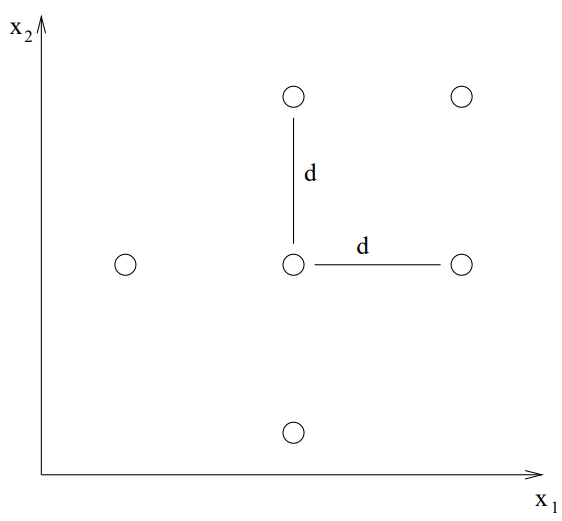
\includegraphics[height=0.6\textheight ,width=0.6\textwidth]{img/17/wyznaczanie_pochodnych}
	\end{figure}
    \begin{block}{}
      poza p.~symetrycznymi potrzeba $\frac{n(n-1)}{2}$ pkt. (mieszane pochodne)
  	\end{block}

  \end{frame}

  \begin{frame}{Metody gradientowe}

    \begin{block}{Metoda największego spadku}
      $\Rightarrow$ podążanie w kierunku wyznaczonym przez - $\vec g$ (gradient)
      \\(w tym kierunku funkcja maleje najszybciej) (Cauchy)
      \\$\left\{
        \begin{array}{l}
          \text{- seria minimalizacji 1-D wzdłuż kierunku największego spadku} \\
          \text{- iteracyjna, bo gradient nie jest stały}
	    \end{array}
	  \right.$
  	\end{block}
    \begin{figure}
		\centering
		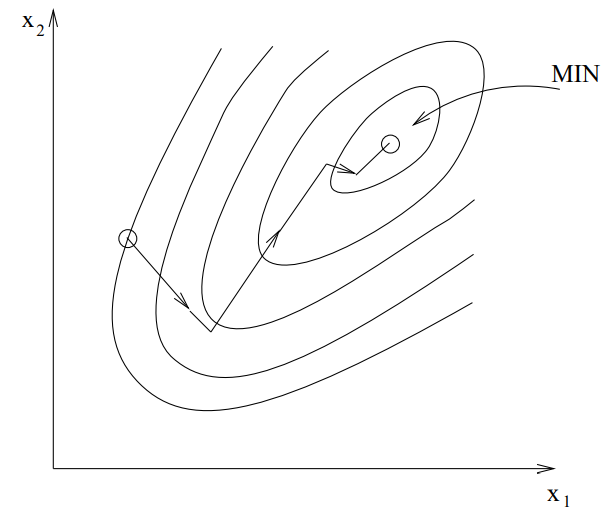
\includegraphics[height=0.5\textheight ,width=0.6\textwidth]{img/17/high_fall_met_1}
	\end{figure}

  \end{frame}

  \begin{frame}{Metoda największego spadku cd.}

    \begin{block}{}
      $\rightarrow$ jeżeli minimalizacja w 1-D 7 dokładna w kierunkach ortogonalnych
      $\Rightarrow$ \emph{met. uzmienniania 1 parametru}
      \smallskip
      \\Łatwo o przykład hipotetycznej funkcji,
      \\ dla której  minimum jest $\perp$ gradientu
  	\end{block}
    \begin{figure}
		\centering
		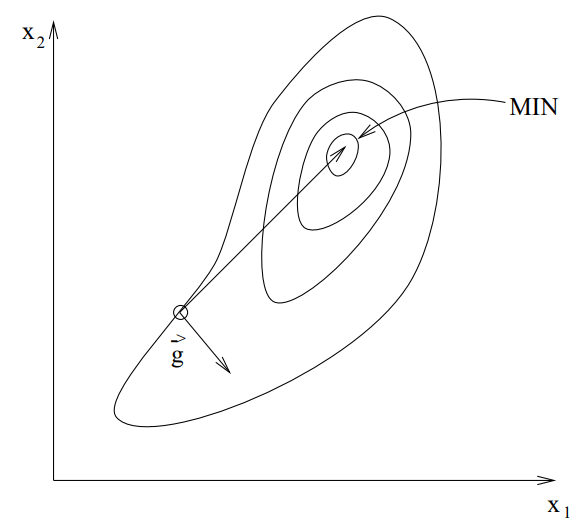
\includegraphics[height=0.5\textheight ,width=0.6\textwidth]{img/17/high_fall_met_2}
	\end{figure}

  \end{frame}

  \begin{frame}{Metody gradientowe}

    \begin{block}{Metoda Newtona}
      Ogólna funkcja kwadratowa jest określona przez:
      \\$\left.
        \begin{array}{l}
          \text{- wartość,} \\
          \text{- pierwsze i} \\
          \text{- drugie pochodne}
	    \end{array}
	  \right\}$
	  $\begin{array}{l} \text{\emph{w dowolnym punkcie }} x_0 \Rightarrow \\ \text{tymi informacjami} \end{array}$
	  \smallskip
	  \\Minimalizacja w pierwszym kroku.
	  \begin{displaymath}
	  		F(\vec{x}) = F(\vec{x_0}) + \vec{g}^T \cdot (\vec{x} - \vec{x_0}) +
	  		\frac{1}{2} (\vec{x} - \vec{x_0})^T \cdot G \cdot (\vec{x} - \vec{x_0})
	  \end{displaymath}
	  $\vec{g} - w \ \vec{x_0} \quad G$ -  stała macierz
	  \smallskip
	  \\Minimum:
	  \begin{displaymath}
	  		\vec{x_m} = \vec{x_0} - G^{-1} \cdot \vec{g} =  \vec{x_0} - V \cdot \vec{g}
	  \end{displaymath}
	\end{block}

  \end{frame}

  \begin{frame}{Metoda Newtona cd.}

    \begin{block}{}
      $\clubsuit Z1$ - sprawdzić: $V = G^{-1}$ -- macierz kowariancji (covariance)
      \\$\Rightarrow$ jest to n-D odpowiednik 1-D interpolacji kwadratowej
      \smallskip
	  \\ \emph{te same wady!}
	  \begin{itemize}
	  	\item[--] niestabilna
	  	\item[--] rozbieżna, gdy $V$ nie jest dodatnio określona
	  \end{itemize}
	\end{block}
    \begin{block}{Zalety:}
      \begin{itemize}
	  	\item[--] krok nie jest dowolny $\rightarrow$ określony przez metodę
	  	\item[--] kierunek $\neq$ gradientu $\rightarrow$ brana pod uwagę korelacja parametrów
	  \end{itemize}
	\end{block}

  \end{frame}

  \begin{frame}{Metoda Newtona cd.}

	\begin{block}{Używana:}
      \begin{itemize}
	  	\item[--] blisko minimum
	  	\item[--] funkcja $\rightarrow$ dodatnia kwadratowa (liniowe najmniejsze kwadraty) % ?????
	  \end{itemize}
	\end{block}
	\begin{block}{}
	    $\Rightarrow$ \emph{Ponadto - podstawa wielu metod}
	\end{block}

  \end{frame}

  \begin{frame}{Metody gradientowe}

    \begin{block}{Dygresja: dodatnio określone formy kwadratowe}
      \emph{1-D forma kwadratowa:}
	  \begin{equation}
	  	F(x) = a + g \cdot x + \frac{1}{2} G \cdot x^2
      \nonumber
	  \end{equation}
    \begin{equation}
      g = \left.\frac{\partial F}{\partial x}\right|_{0}{,}\qquad
      G = \left.\frac{\partial^{2} F}{\partial x^2}\right|_{0}
      \nonumber
    \end{equation}
	  $F(x)$ ma min. wtedy i tylko wtedy, gdy $G$ $\geq 0$.
    \begin{equation}
	  		G = 0 \rightarrow \text{\emph{min}} \rightarrow \infty; \qquad
        x^m = -g/G
        \nonumber
	  \end{equation}
	  \emph{Dla ogólnej funkcji nieliniowej:}
	  \smallskip
	  \begin{itemize}
	  	    \item krok do $x = \frac{g}{G}$ gdy $G > 0$
	  	    \\(w przeciwnym przypadku: $\infty$ lub maximum)
	  \end{itemize}
	\end{block}

  \end{frame}

  \begin{frame}{Dodatnio określone formy kwadratowe cd.}

    \begin{figure}
		\centering
		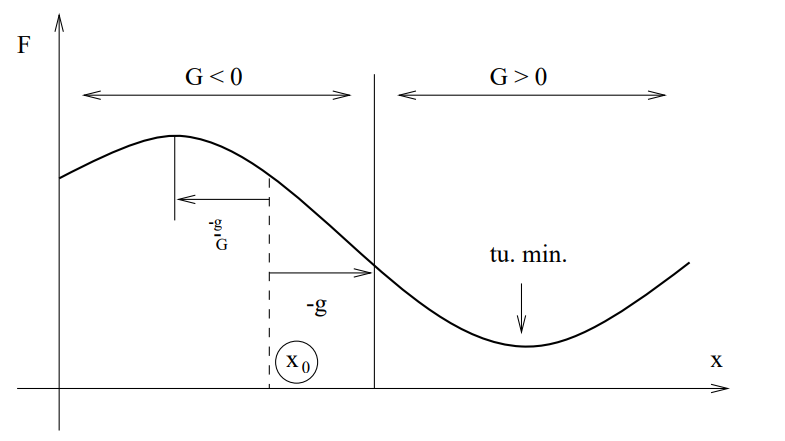
\includegraphics[width=0.95\textwidth]{img/17/dygresja}
	\end{figure}

  \end{frame}

  \begin{frame}{Dodatnio określone formy kwadratowe cd.}

    \begin{block}{}
    	\begin{itemize}
	  	    \item gdy $G \leq 0$ krok $= -g$
	  	    \\$\rightarrow$ kierunek - dobry,
	  	    \\$\rightarrow$ wartość - dowolna
	    \end{itemize}
	    W $x_0 \rightarrow F(x)$ nie jest wypukła (dodatnio określona)
	    \medskip\\
	    \emph{Uogólnienie na n-D:}\\
	    $g \rightarrow \vec{g}$, $G$ - macierz 2-ich poch.;
	    $F(\vec X) = a + \vec{g}^T \cdot \vec{x} + \frac{1}{2} \vec{x}^T G$ tylko dla $G$ dod. określonej
	    ma sens krok do:
	    \begin{displaymath}
	  		\vec{x} = - G^{-1} \cdot \vec{g}
	    \end{displaymath}
    \end{block}

  \end{frame}

  \begin{frame}{Metody gradientowe}

    \begin{block}{Badanie czy $G$ jest dodatnio określona}
      \begin{itemize}
      		\item[--] brak prostych sposobów
      \end{itemize}
    \end{block}
    \begin{block}{\emph{Dla macierzy kwadratowych, symetrycznych - 2 warunki konieczne}}
      $1^o$ elementy diagonalne $> 0$ \ (wyst. 1 $\times$ 1)
      \\$2^o$ elementy pozadiagonalne:
      \begin{displaymath}
      		G_{ij}^2 < G_{ii} \cdot G_{jj}
      \end{displaymath}
    \end{block}

  \end{frame}

  \begin{frame}{Badanie czy $G$ jest dodatnio określona cd.}

    \begin{block}{Ogólne warunki konieczne i wystarczające}
      \begin{itemize}
      		\item[--] wszystkie wartości własne $> 0$ (b. trudne i przybliżone)
      		\item[--] wyznacznik wszystkich macierzy $> 0$
      		\begin{figure}
				\centering
				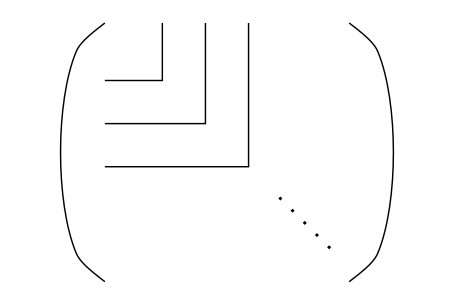
\includegraphics[height=0.2\textheight ,width=0.3\textwidth]{img/17/matrix}
			\end{figure}
			(najprościej sprawdzić)
			\item[--] skalar $E^T \cdot G\vec{e} > 0$ dla $\bigwedge \vec{e}$ (zwykłe $\rightarrow$ def.), wyjaśnia dlaczego $G$ dod.
			okr. daje formę $F(x)$ z minimum: $F(x)$ rośnie we wszystkich kierunkach od $\vec{e} = 0$
			\item[--] $-V = G^{-1}$ jest dodatnio określona
      \end{itemize}
    \end{block}

  \end{frame}

  \begin{frame}{Metody gradientowe}

 	\begin{block}{Postępowanie w przypadku $G$ - nie jest dod. określone}
 	   \begin{enumerate}[a)]
 	   		\item analogicznie do 1-D : G = I $\rightarrow$ Ale:
 	   		\item lepiej:
 	   		\begin{itemize}
 	   			\item[--] gdy $\bigwedge$ elementy diagonalne $G > 0$, wtedy pozadiag. $\rightarrow = 0$ (scale - invariant step),
 	   			\item[--] gdy tylko niektóre el. pozadiag. $G_{ij}^2 \geq G_{ii}G_{jj} \Rightarrow G_{ij} = 0$,
 	   			\item[--] zamiast $G^{-1}$ bierzemy $(G + \lambda \cdot I)^{-1}$;
 	   			\\ $\lambda \geq$ największa (bezwzgl.) ujemna wartość własna:
 	   			\begin{itemize}
 	   				\item[--] dużo obliczeń,
 	   				\item[--] krok pośredni pomiędzy m. Newtona a największego spadku
 	   				\\(duże $\lambda$ : krok krótki, w kierunku $\vec{g}$)
 	   			\end{itemize}
 	   			\item[--] gdy jedna lub więcej diagonalnych 2-ich poch. $< 0$
 	   			\\ $\Rightarrow$ informacja o kierunku wzrostu ujemnej 1-szej poch.
 	   			\\w tym kierunku - szukanie met. zmiany 1 param.
 	   		\end{itemize}
 	   \end{enumerate}
 	\end{block}

  \end{frame}

  \begin{frame}{Gdy $G$ - nie jest dodatnio określone cd.}

 	\begin{block}{}
 	Metody oparte na powyższych regułach - \emph{quasi-Newton m.}
 	\medskip
 	\\Podstawowa wada tych metod - obliczanie i odwracanie
 	\\w każdym kroku macierzy drugich pochodnych
 	\smallskip
 	   	\begin{itemize}
 	   		\item[--] obliczanie 2-ich poch. $\sim n^2$ (długie)
 	   		\item[--] odwracanie
 	   	\end{itemize}
 	\end{block}

  \end{frame}

  \begin{frame}{Metody gradientowe}

 	\begin{block}{Metoda sprzężonych kierunków \emph{conjugate directions}}
 	   Wektory $\vec{d_i}$ i $\vec{d_j}$ \emph{są sprzężone} ze względu na dodatnio określoną macierz, jeżeli:
 	   \\$\vec{d_i}^T A\vec{d_j} = 0$ dla $i \neq j$;
 	   \\gdy $A = I, \vec{d_i} \rightarrow$ ortogonalne
 	   \\(sprzężenie - uogólnienie ortogonalności)
 	   \\ \textbf{$n$ sprzężonych wektorów rozpina n-D przestrzeń}.
 	   \\$A$ - nie określa jednoznacznie zbioru wektorów sprzężonych $\rightarrow$ można zastosować
 	   \emph{uogólnienie procedury ortogonalizacji Grama-Schmidta}:
 	   \\$d_1$ - dowolny wektor $d_2 = A \cdot d_1 - \frac{d_1^T A A d_1}{d_1^T A d_1} \cdot d_1 \rightarrow$ sprzężony do $d_1$
 	   \\$d_3 =$ \ldots
 	   \begin{flushright}
 	      $\clubsuit$ sprawdzić
 	   \end{flushright}
 	\end{block}

  \end{frame}

  \begin{frame}{Metoda sprzężonych kierunków cd.}

    W minimalizacji - użyteczne wektory sprzężone
    \\ze względu na \emph{hesjan} $G$
 	\begin{block}{Twierdzenie}
 	   Sekwencja liniowych minimalizacji w każdym z $n$ sprzężonych kierunków minimalizuje ogólną funkcję kwadratową $n$ zmiennych.
 	\end{block}
 	\begin{block}{Dowód:}
 	   $\left\{
        \begin{array}{l l}
          \text{funkcja:} & F(\vec{x}) = F(\vec{0}) + \vec{g}^T \vec{x} + \frac{1}{2} x^T G \vec{x} \\
          \text{kierunki sprzężone:} & \vec{d_i} \ \vec{d_i}^T G \vec{d_j} = 0 \ i \neq j
	    \end{array}
	  \right.$
	  \\gdzie: $G$ jest macierzą
 	\end{block}

  \end{frame}

  \begin{frame}{Metoda sprzężonych kierunków cd.}

 	\begin{block}{Dowód cd.}
		\emph{$x, g$ -  jako kombinacje liniowe:} w układzie o wektorach jednostkowych
		\begin{displaymath}
			\vec{x} = \sum_i y_i \vec{d_i}, \quad \vec{g} = \sum_i c_i \vec{d_i}
		\end{displaymath}
		wtedy:
		\begin{displaymath}
			F(x) = F(0) + (\sum_i c_i \vec{d_i}^T) \cdot (\sum_j y_j \vec{d_j}) +
			\underbrace{\frac{1}{2} (\sum_i y_i \vec{d_i}^T) \cdot G \cdot (\sum_j y_j \vec{d_j})}_{(\star)}
		\end{displaymath}
 	\end{block}

  \end{frame}

  \begin{frame}{Metoda sprzężonych kierunków cd.}

 	\begin{block}{Dowód cd.}
 		($\star$) wynik przegrupowania $\Rightarrow$
		\begin{itemize}
			\item podwójna suma
			\item $i \neq j \Rightarrow$ równe zero (warunek sprzężenia)
		\end{itemize}
		\begin{displaymath}
			F(x) = F(0) + \sum_i \sum_i c_i d_i^T d_j y_j + \frac{1}{2} \sum_j y_j^2 d_j^T G d_j =
		\end{displaymath}
		\begin{center}
		   	\begin{tabular}{|c|}
		   	\hline
				$F(0) + \sum_j (b_j y_j + b'_j y_j^2)$
			\\ \hline
			\end{tabular}
			\smallskip
			\\gdzie:
			\begin{tabular}{|c|}
		   	\hline
				$b_j = \sum_i c_i d_i^T d_j{,} \quad b'_j = \frac{1}{2} d_j^T G d_j$ - \underline{stałe}
			\\ \hline
			\end{tabular}
		\end{center}
		\emph{zamiast} $\vec{x}$ \emph{- mamy} $\vec{y}$, przy czym $F(x)$ stała się \emph{sumą niezależnych jednoparametrowych} funkcji kwadratowych. Minimalizacja ze względu na $y_i$ (wzdłuż kierunku $\vec{d_i}$) jest niezależna od minimalizacji  względem pozostałych sprzężonych kierunków.
 	\end{block}

  \end{frame}

  \begin{frame}{Metoda sprzężonych kierunków cd.}

 	\begin{block}{Wnioski:}
		\begin{itemize}
			\item[--] minimalizacja nie wzdłuż osi ortogonalnych,
			\\ale wzdłuż kierunków sprzężonych
		\end{itemize}
 	\end{block}
 	\begin{block}{}
		Ale $\Rightarrow$ szukać innej konstrukcji $d_i$ \emph{(gdy znamy $G$ - m. Newtona
		\\- w 1 kroku!)} $\Rightarrow$ \emph{Można wyznaczyć $d_i$ bez $G$!}
 	\end{block}
 	\begin{block}{Twierdzenie}
		Jeżeli $\vec{x_0}, \vec{x_1}$ - punkty min. w 2 równoległych podprzestrzeniach,
		\\to $(\vec{x_1} - \vec{x_0})$ jest sprzężony do każdego wektora w tych dwóch podprzestrzeniach.
 	\end{block}

  \end{frame}

  \begin{frame}{Metoda sprzężonych kierunków cd. }

 	\begin{block}{Dowód}
	  $\vec{x_0}$ - min. wzdłuż $d_i$; to gradient F w $\vec{x_0}$ musi być $\perp \vec{d_1}$
	  \smallskip
	  \begin{center}
	    $ \left\{
          \begin{array}{l}
            \vec{d_1}^T \cdot (\vec{g} + G \vec{x_0}) = 0 \\
            \vec{d_1}^T \cdot (\vec{g} + G \vec{x_1}) = 0
	      \end{array}
	    \right\} $
	    \ $(\vec{g}$ \emph{grad. w} $x = 0)$
	  \end{center}
	  \begin{center}
	    $\vec{d_1}^T \cdot G (\vec{x_1} - \vec{x_0}) = 0 \qquad (\vec{x_1} - \vec{x_0})$ sprzężony do $\vec{d_1}$
	  \end{center}
 	\end{block}

  \end{frame}

  \begin{frame}{Metoda sprzężonych kierunków cd. }

   \begin{block}{Dowód cd.}
	  w przestrzeni:
	  \smallskip
	  \\3-D $\Rightarrow$ 3 dodatkowe minimalizacje
	  \\ \ (3-ci kier. sprzężenia do 2 pierwszych)
	  \\n-D $\Rightarrow$ $\frac{n(n+1)}{2}$ minimalizacje - ile elem. w $G$ - ale:
	  \\ \ met. b. stabilna dla $F(x) \neq$ kwadratowych i nie wymaga
	  \\ \ znajomości pochodnych
	  \medskip
	  \\Uwaga: \emph{asymetria:}
	  \begin{itemize}
	  	  \item $n$ minimal. w $d_1$
	  	  \item $1$ minimal. w $d_n$
	  \end{itemize}
 	\end{block}

  \end{frame}

  \begin{frame}{Metody gradientowe}

 	\begin{block}{Metoda gradientów sprzężonych \emph{(conjugate gradients)}}
 	   $\Rightarrow$ wykorzystuje tylko 1-sze pochodne.
 	   \medskip
 	   \\ $F(\vec{x})$ i $\vec{g}(\vec{x})$ wyznaczone w $\vec{x_0}$ i $\vec{x_1}$, z nich:
 	   \smallskip
 	   \\ $\vec{\Delta x} = \vec{x_1} - \vec{x_0}$, \ $\vec{\Delta g} = \vec{g_1} - \vec{g_0}$
 	   \smallskip
 	   \\ Dla $F(\vec{x})$ kwadratowej, z hesjanem $G$:
 	   $\begin{array}{|c|}
 	   	  \hline
 	   	  \vec{\Delta g} = G \cdot \vec{\Delta x}
 	   	  \\ \hline
 	   \end{array}$,
 	   \\zatem dowolny $\vec{d_1} \perp \vec{\Delta g}$ będzie dodany do $\vec{\Delta x}$:
 	   \begin{center}
 	      $\begin{array}{|c|}
 	   	    \hline
 	   	    \vec{d_1}^T \cdot \vec{\Delta g} = \vec{d_1} G \vec{\Delta x} = 0
 	   	    \\ \hline
 	      \end{array}$
 	   \end{center}
 	   \smallskip
 	   $\Rightarrow$ metoda uzyskiwania kierunków sprzężonych \emph{bez} znajomości $G$:
 	   \\Pierwszy kierunek: $\vec{d_0} = \vec{-g_0}$
 	   \\min. wzdłuż $\vec{d_0}$ : w $\vec{x_1}$, gradient:  $\vec{g_1}$
 	   \\Drugi kierunek: $\vec{d_1} = -\vec{g_1} + b \cdot \vec{d_0}$
 	   \\(liniowa kombinacja znanych kierunków)
 	\end{block}

  \end{frame}

  \begin{frame}{Metoda gradientów sprzężonych cd. }

   \begin{block}{}
	  Warunek sprzężenia: $\vec{d_1}^T \cdot G \cdot \vec{d_0} = \vec{d_1}^T \cdot G \cdot (\vec{g_1} - \vec{g_0}) = 0$, czyli:
	  $(-\vec{g_1} + b \cdot \vec{d_0}) \cdot G \cdot \vec{d_0} = (-\vec{g_1} -b \cdot \vec{g_0}) \cdot (\vec{g_1} - \vec{g_0}) = 0$
	  \\$\vec{x_1}$ - to min. wzdłuż $\vec{d_0} = -\vec{g_0} \Rightarrow \vec{g_0} \perp \vec{g_1} : \vec{g_1}^T \cdot \vec{g_0} = 0$
	  \smallskip
	  \\$\Rightarrow$
	  $\begin{array}{|c|}
 	   	 \hline
 	   	    b = \frac{\vec{g_1}^T \cdot \vec{g_1}}{\vec{g_0}^T \cdot \vec{g_0}}
 	   	 \\ \hline
	  \end{array}$,
 	  czyli nowy sprzężony kierunek $\vec{d_1} = -\vec{g_1} + \left(\frac{\vec{g_1}^T \cdot \vec{g_1}}{\vec{g_0}^T \cdot \vec{g_0}}\right) \cdot \vec{d_0} $
 	  \medskip
 	  \\i ten proces kontynuujemy generując $n$ kierunków \\ wzajemnie sprzężonych.
 	  \medskip
 	  \\Można pokazać, że dla wszystkich sprzężonych kierunków zachodzi:
 	  \begin{center}
 	  	 $\begin{array}{|c|}
 	   	   \hline
 	   	      \vec{d_{i+1}} = -\vec{g_{i+1}} + \frac{\vec{g_{i+1}}^T \cdot \vec{g_{i+1}}}{\vec{g_{i}}^T \cdot \vec{g_{i}}} \cdot \vec{d_i}
 	   	   \\ \hline
	    \end{array}$
 	  \end{center}
 	\end{block}

  \end{frame}
